\documentclass{beamer}

\usetheme[bgphoto]{polimi}
\usefonttheme[onlymath]{serif}

% Full instructions available at:
% https://github.com/elauksap/beamerthemepolimi

% Set custom font (requires to compile with XeLaTeX).
\usepackage{ifxetex}
\ifxetex
    \usepackage{fontspec}
    \setsansfont[Scale=0.95]{Arial}
\fi

\usepackage{lipsum}

\title{Title}
\subtitle{Subtitle}
\author{Author}
\date{dd mm yyyy}

\begin{document}
    \begin{frame}
        \maketitle
        % If the theme option "nologo" is specified, a custom logo
        % can be added with the following commands:
        %\begin{tikzpicture}[overlay, remember picture]
        %    \node at (current page.north) [anchor=north, inner sep=2cm]
        %    {
        %        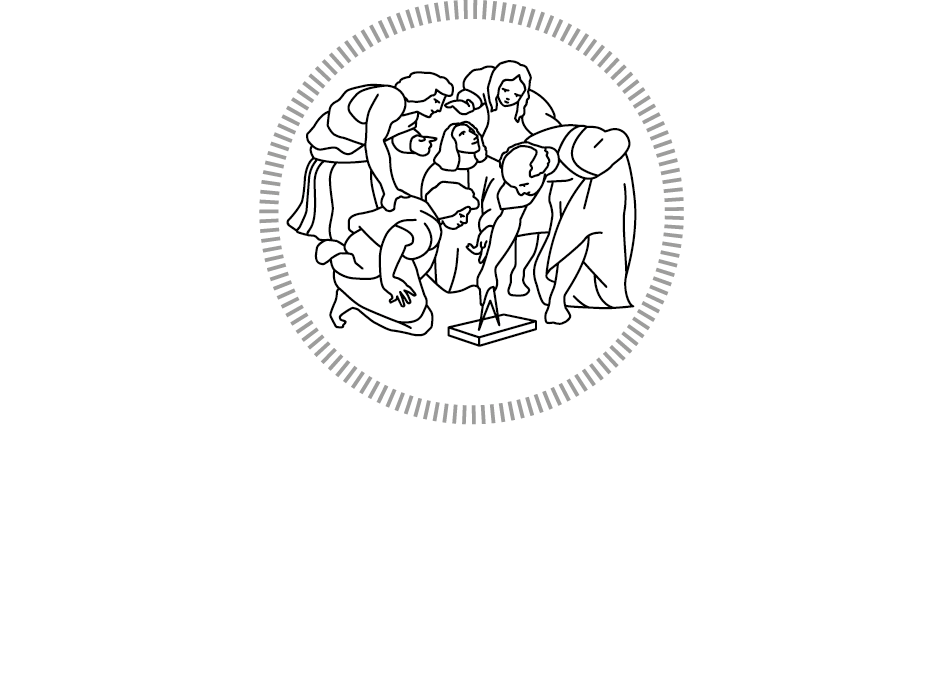
\includegraphics[width=0.3\paperwidth]{logo_centrato_BN_negativo.png}
        %    };
        %\end{tikzpicture}
    \end{frame}
    
    \begin{frame}{Outline}
      \tableofcontents
    \end{frame}
    
\section{Objective}
    % Section page.
    \begin{frame}[plain]{}
        \sectionpage
    \end{frame}
    
    \begin{frame}{Initial Research Question}
        \begin{block}{Lagrangian Particle Tracking of Snowflakes}
        	Find a general formula for the drag coefficient of blowing snow
        	\begin{equation*}
        		c_D = c_D (Re, \text{parameters})
        	\end{equation*}
        	And implement it in PoliMIce with some general rule for the choice of the main parameters.
        \end{block}
    \end{frame}
    
    \begin{frame}{Literature Review}
    	\begin{alertblock}{What is not available}
    		\begin{itemize}
    			\item $ c_D $ formula tuned for snowflakes
    			\item Experimental measurements of blowing snowflakes velocities
    			\item Shape of the typical snowflake (they are almost unique)
    		\end{itemize}
    	\end{alertblock}
    
		\begin{exampleblock}{What is available}
			\begin{itemize}
				\item $ c_D $ formulae tuned for arbitrary shaped bodies
				\item Experimental measurements of falling snowflakes terminal velocities
				\item General parameters that describe the shape (CAMBIARE)
			\end{itemize}
		\end{exampleblock}
    \end{frame}

    \begin{frame}{Updated Research Question}
		\begin{block}{Drag coefficient formula}
			Find a suitable existing model to infer the main parameters in the falling regime and use them in the blowing one
		\end{block}
	
		\begin{block}{Snow Parameters}
			Develop a method to find the discrete set of properties that on average describe a certain \textit{cloud}
		\end{block}
	\end{frame}
    
\section{Method}
    \begin{frame}{Outline}
    	\tableofcontents[currentsection]
    \end{frame}
    
    \begin{frame}{Data Generation}
		Reproduce an artificial data set from the \textit{velocity-diameter} relation of Brandes et al - 2008. The diameter distribution is not taken into account.
		
		\centering
		
\includegraphics[height=.5\textheight]{404notFound.png}
    \end{frame}

\subsection{Data Analysis}
	\begin{frame}{The Drag Model}
		\begin{block}{Ganser - 1993}
			\begin{equation*}
				c_D = K_2 \left( \frac{24}{Re K_1 K_2} (1 + 0.1118 (Re K_1 K_2)^{0.6567}) + \frac{0.4305}{1 + \frac{3305}{Re K_1 K_2}}\right) 
			\end{equation*}
			\vfill
		\end{block}
		
		
		\begin{columns}[T]
			\begin{column}{.4\textwidth}
				\begin{block}{Stokes' Shape Factor}
					\centering
					$ K_1 = \left( \frac{1}{3} \frac{d_n}{d_v} + \frac{2}{3} \Phi^{-\frac{1}{2}} \right)^{-1} $
				\end{block}
			\end{column}
			
			\begin{column}{.4\textwidth}
				\begin{block}{Newton's Shape Factor}
					\centering
					$ K_2 = 10^{1.8148 (-log(\Phi))^{0.5743}} $
				\end{block}
			\end{column}
		\end{columns}
	\end{frame}

	\begin{frame}{General Scheme}
		\begin{columns}[T]
			\begin{column}{.4\textwidth}
				\centering
				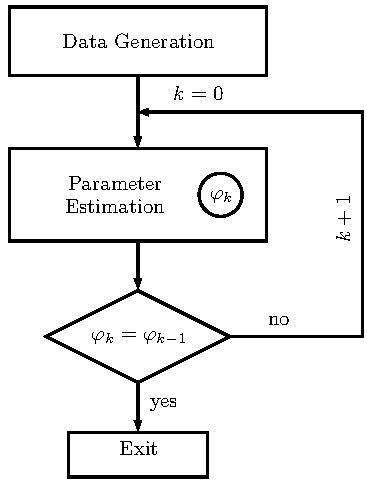
\includegraphics[height=.6\textheight, keepaspectratio] {GeneralScheme.pdf}
			\end{column}
		
			\begin{column}{.6\textwidth}
				\centering
				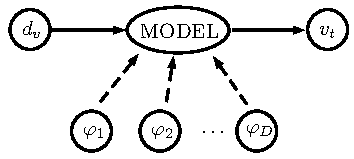
\includegraphics[width=.9\textwidth, keepaspectratio] {MultiParameter.pdf}
				\begin{itemize}
					\item $ (d_v, v_t) $: Experimental data
					\item $ \varphi_1, \varphi_2 \dots \varphi_D = \underline{\varphi} $: Free parameters
					\item $ D $: Number of parameters $ \sim  $ problem dimension
				\end{itemize}
			\end{column}
		\end{columns}
	\end{frame}

	\begin{frame}{Bayesian Approach}
		\begin{block}{Bayes' Theorem}
			\begin{equation*}
				\underbrace{prob(\delta HP|D,I)}_{Posterior Probability} \propto
				\underbrace{prob(D|\delta HP,I)}_{Likelihood Function} \cdot \underbrace{prob(\delta HP|I)}_{Prior Probability}
			\end{equation*}
			\begin{itemize}
				\item \textit{Prior:} State of knowledge (or ignorance) before analyzing the data 
				
				\item \textit{Likelihood:} Experimental measurements
				\item \textit{Posterior:} State of knowledge in light of the data
			\end{itemize}
		\end{block}
	
	
		\begin{block}{Marginalization Equation and Sum Rule}
			\begin{equation*}
				prob(HP|D,I) = \int_{-\infty}^{+\infty} prob(\delta HP|D,I) \delta HP = 1
			\end{equation*}
		\end{block}
	\end{frame}
	
	\begin{frame}{Problem formulation}
		\begin{block}{Prior}
			\begin{equation*}
				\begin{split}			
				prob(HP|I) & = prob(\underline{\varphi}) : \textit{Uniform} \text{ in the range of physical solution.}\\
				& = \left\{ 
				\begin{array}{cc}
				\dfrac{1}{(\varphi_{1, M} - \varphi_{1, m}) (\varphi_{2, M} - \varphi_{2, m}) \dots (\varphi_{D, M} - \varphi_{D, m})} \\
				0 
				\end{array} \right.
				\end{split}
			\end{equation*}				
		\end{block}
		
		\begin{block}{Likelihood}
			\begin{equation*}
				prob(D|HP,I) = \prod_{n = 1}^{N_{data}} \sum_{k = 1}^{N_{modes}} \pi_k \ e^{-\dfrac{1}{2} \left(\dfrac{v_{t,n} - v_t(d_{v,n}, \underline{\varphi}_k)}{\sigma_n} \right)^2}
			\end{equation*}
		\end{block}	
	\end{frame}

	\begin{frame}{Gaussian Mixture Models}
		\centering
		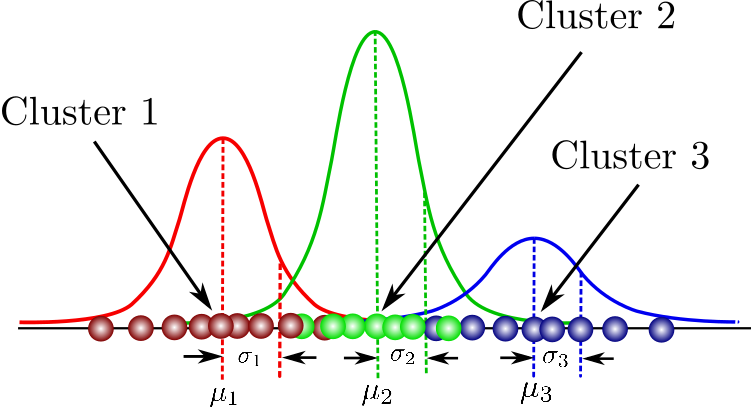
\includegraphics[height=.6\textheight]{GMM.png}
	\end{frame}

\section{Result}
	\begin{frame}{Brandes}
		\centering
		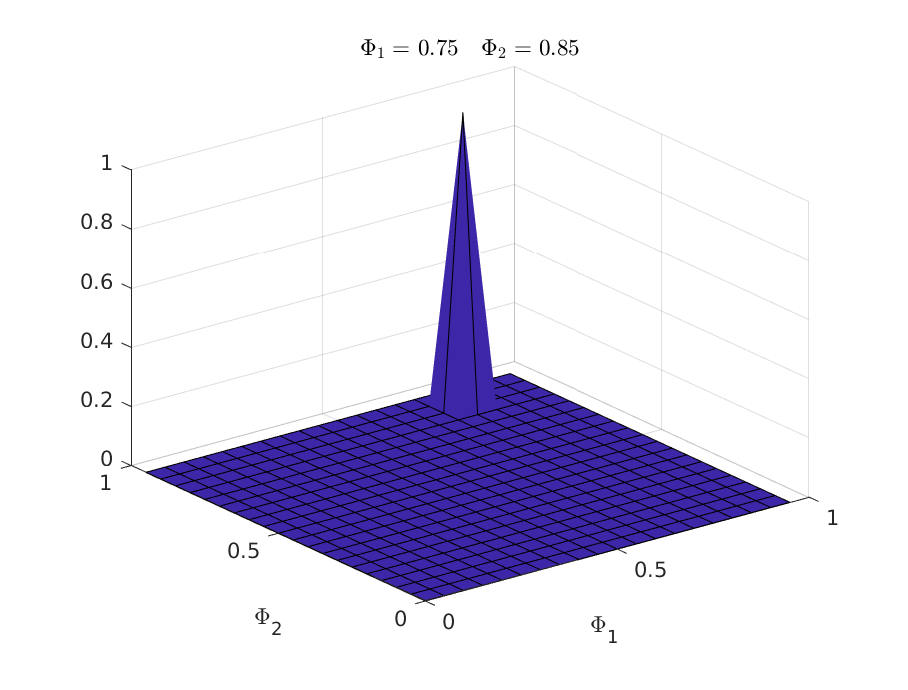
\includegraphics[height=.6\textheight]{Brandes11.eps}
	\end{frame}


\end{document}
